\chapter{Introduction}
\label{ch:chapter_1}

%% The following annotation is customary for chapter which have already been
%% published as a paper.
%\blfootnote{Parts of this chapter have been published in Annalen der Physik \textbf{324}, 289 (1906) ~\cite{Einstein1906}.}

%% It is only necessary to list the authors if multiple people contributed
%% significantly to the chapter.
%\authors{Albert {\titleshape Einstein}}

%% The '0pt' option ensures that no extra vertical space follows this epigraph,
%% since there is another epigraph after it.
%\epigraph[0pt]{
%    "Stories of imagination tend to upset those without one."
%}{Sir Terry Pratchett}

\epigraph{
    “Did I mention that I know almost everything about almost everything ?”
}{Dr. Rodney McKay, fictional character}

\begin{abstract}
Molecular electronics is a relatively young field that attempts to find functional molecular junctions as a logical extension of the minimisation of semiconductors. Both theoretically and experimentally, great progress has been made since its inception but there is still sufficient room for more progress. 
\end{abstract}

%% Start the actual chapter on a new page.
\newpage
\section{Molecular Electronics}
Modern electronics is almost entirely based on semiconductor physics. The most abundant and thus primary element is silicon. Since the 1960, efforts have been made to minimise the semiconductor devices to ever smaller scales. However, semiconductors are a `bulk' approximation. Now that the downsizing approaches molecular scales, it is at its end ~\cite{seldenthuis}.

The next smallest functional element is a molecule. Evolution by natural selection has, at the biochemical scale, led to a very broad spectrum of functional molecules. We can synthesise a great amount of molecules simply by utilising the specialised enzymes provided in that way.

At the molecular scale, new functionality also arises. For instance, molecules can respond to light and heat. They can act as logic gates, rectifiers, solar cells and much more ~\cite{perrin}. 

Experts see the most exciting future of the field in that direction, in new functional elements rather than replacement of semiconductor elements ~\cite{visions}.

Fundamental to the creation of nanoscopic devices is the understanding of both the behaviour and the fabrication. My thesis focuses almost entirely on the first aspect, albeit previous experiments will be discussed as a way of confirming or motivation theoretical work.

On the experimental side, various aspects are quite involved. For instance, the reproducible contacting of a single-molecule in a device is far from easy. As a result, statistical approaches to measure conductance and other molecular properties are essential. The challenge lies partially in reducing the variability or to exploit molecular functionalities that are insensitive to the details of the contacts ~\cite{visions}.

For theory, on the other hand, the challenge lies in removing the mismatch between theory and experiment. In particular, predicting transport gaps and determining the Fermi energy have proven very challenging~\cite{perrin}. 

Primarily we focus on incorporating interactions into the formalism. Normally, only single-electron transport is considered, partially because the appropriate formalism  was not available. Starting from a note by Dr. Jos Seldenthuis, we develop the appropriate formalism. We apply this to a model that has been shown to qualitatively work well to explain the behaviour of thiolated arelythynylene with a dihydroanthracene core ~\cite{perrinnano}. We also consider a novel version of that model that incorporates spin. 
%%%%%%%%%%%%%%%%%%%%%%%%%%%%%%%%%%%%%%%%%%%%%%%%%%%%%%%%%%%%%%%%%%%%%%%%%%%%%%%%%%%%%%%%%%%%%%%%%%%%%%%%%%%%%%%%%%%%%%%%%%%%%%%%%
\section{Experimental}
I will shortly review a number of the more popular techniques for single-molecule experiments. To wit, these are Atomic Force Microscopy (AFM), Scanneling Tunneling Microscopy (STM), Electromigration and finally Mechanically Controlled Break Junctions (MCBJ). I think it important to have some knowledge of the experimental reality of the nanoscopic devices I investigate theoretically.

\index{Atomic Force Microscopy} is a type of scanning probe microscopy with resolution of less than a single nanometre. By using a piezoelectric element, it can make an incredibly accurate surface scan by keeping the forces between probe and sample constant~\cite{frei1, frei2}.

For molecular electronics, molecules are evaporated onto the gold substrate. The AFM tip, a golden cantilever, is brought into contact with a substrate and slowly retracted. The evaporated molecules form a self-assembled mono layer, so that some molecules have migrated onto the substrate-tip bond. As it breaks, a molecular break junction is formed.

The AFM method has several advantages. First, it can measure both electrical current and forces in a parallel measurement~\cite{nef}. Another large advantage is that the topographic imaging and electrical measurement are simultaneously achieved, so that the nano-device is relatively well documented before measurement ensues.

The \index{Scanneling Tunneling Microscopy} method features similar advantages \cite{Joachim2000}, but instead of using a golden cantilever it is the scanning probe tip that is brought into contact with a molecule, and then very slowly pulled away. The molecule, which bonds to the tip, is the stretched between the substrate and the STM tip, making another (gold) molecular junction.

\index{Electromigration} is a method of gap formation that is conceptually interesting. An overlapping set of gold leads is made, which is put through voltage ramps at ambient laboratory conditions. The voltages increase the mobility of the gold atoms, which move away from the future gap. The gap formed by this method is reproducible~\cite{electromigration}.

Finally, the \index{Molecular Controlled Break Junction} is the technique used by~\citet{perrinnano}, which we will discuss later in section~\ref{sec:perrin}. Most of the following descriptions is based on~\citet{perrin} or conversations with him. In figure~\ref{fig:mcbj} the basic setup of a Mechanically Controllable Break Junction (MCBJ) is shown. These offer high electrode stability and fine-tuning of the electrode spacing. 
\begin{figure}[!bp]
    \centering
    \includegraphics[height=0.3\textheight,page=2, clip=true, trim=2.5cm 16.5cm 11cm 6cm]{pdf/perrinnnano.pdf}
    \caption{Schematic drawing of a MCBJ. A Gold wire is deposited on top of a flexible substrate, which is then bend by the three-point mechanism. The wire breaks, forming a size-controllable gap.}
    \label{fig:mcbj}
\end{figure}

The working principle behind the MCBJ technique is to deposition a thin metallic wire on top of a flexible substrate. Here, gold is used because it is a noble metal. By bending the substrate in a three-point mechanism, the gold wire stretches and breaks. It then forms two gold surfaces, the electrodes. The spacing between these electrodes can be tuned by adjusting the bending of the sample. The junction can be reformed after it is broken.

The allowed voltage over such a MCBJ junction ranges from $0.5$ V at room temperature up to $2$-$3$ V at $4.2$K. At low temperatures, the size of the gap does not significantly change over time. Additionally, the technique allows repeated fusing and breaking, and is thus ideal for statistical studies which are required for mechanistic insight because of the dominance of large fluctuations in experiments \cite{ratnerrev2013}.

A number of \index{experimental findings}~\cite{koole} regarding electron transports are the Coulomb blockade~\cite{Park2000, Park2002}, the Kondo effect~\cite{Park2002}, vibrational excitations~\cite{vib1, vib2} and electronic excitations~\cite{elec1}.

\section{Theory}
While we work primarily in the non-equilibrium Green's Function Formalism (chapter~\ref{ch:chapter_2}), here I will also briefly describe another formalism often used, namely the Master Equation approach \cite{seldenthuis}. One very large benefit of the Master Equation approach over the non-equilibrium Green's Function approach is that it allows simple conceptual thinking.

I will also give a short description of Density Functional Theory (DFT), a method often used with the non-equilibrium Green's Formalism which will be discussed and derived in analytical detail in chapter~\ref{ch:chapter_2}  .

Let us start by noting that molecules are often considered as quantum dots. If we consider a very simple chain of carbon atoms, with transport dominated by a single molecular orbital, it makes conceptual sense that we can describe this chain with the simplified model of a chain of quantum dots with a single level at that same energy. If we include spin, we could even describe it as a chain of qubits.

The typical way of physicist thinking is the \index{Master Equation} (ME) approach. If we consider one of these dots centred between two others ($c$) , we need to know the rate at which electrons leave it to either the right ($r$ or the left ($l$) neighbouring dot, and the rate at which they enter. Of course, that depends on the chances the neighbouring dots are occupied. Based on this simple reasoning, we can formulate the Master Equation \cite{beenakker}:
\begin{align*}
\partial_t P_c &= P_l W_{l\rightarrow c} - P_c W_{c\rightarrow l} + P_r  W_{r\rightarrow c} - P_c W_{c\rightarrow r}
\end{align*}

Of course, we do not yet know the rates of leaving and entering the centre dot. However, note that the master equation is linear and can be written in matrix form, $\dot{P} = W P$. We use the \index{Born-Oppenheimer approach}, where we assume the wave-function $\ket{\Psi}$ is separable into the atomic nuclei $\ket{\phi}$ and the electronic $\ket{\psi}$. The rates due to a (weak) interaction $H'$ be found from the well-known \index{Fermi's Golden rule} between initial state $\ket{i}$ and final state $\ket{f}$:
\begin{align*}
W_{i\rightarrow f} &= \frac{2\pi}{\hbar} \left| \braket{\phi_f \psi_f \left|H'\right| \phi_i \psi_i}\right|^2 \rho_f (\epsilon_f)
\end{align*}

The atomic overlap $\left| \braket{ \phi_f | \phi_i }\right|^2$ is known as a Franck-Condon factor. Note that different electronic eigenstates very often have a slightly different atomic state, which means that the Franck-Condon factor between non-identical states become non-zero. Theoretically, this can be understood as a basis change; $\ket{\phi_i}$ and $\ket{\phi_f}$ are no longer pure eigenstates in the new basis. 

The ME approach is very suited to handling vibrational excitations and interactions up to any desired order \cite{seldenthuis}. However, it is most suited when electronic interactions are weak, and vibrational interactions are strong. The non-equilibrium Green's Formalism (chapter~\ref{ch:chapter_2}) is its opposite, and is more suited to strong electronic interactions where vibrational coupling can be mainly ignored. 

I will now describe \index{Density Functional Theory} (DFT) as it pertains to transport calculations for single-molecule junctions. 


\section{A brief history of molecular electronics}
It seems both pertinent and interesting to review some of the triumphs of the field. Here, I present a synthesis of experimental and theoretical triumphs.


\section{Outline of thesis}
\references{dissertation}